% Focused Methods + Results manuscript for kidney transplant graft failure prediction
\documentclass[11pt,a4paper]{article}
\usepackage[utf8]{inputenc}
\usepackage[margin=1in]{geometry}
\usepackage{graphicx}
\usepackage{amsmath}
\usepackage{booktabs}
\usepackage{float}
\usepackage{caption}
\usepackage{subcaption}
\usepackage{hyperref}
\usepackage{natbib}
\usepackage{setspace}
\usepackage{multirow}

\onehalfspacing
\graphicspath{{step24_figures/}{step25_figures/}{step30_figures/}{step31_figures/}{step32_figures/}}

\title{Methods and Results: Machine Learning Prediction of Kidney Graft Failure Using UNOS STAR Registry Data}
\author{Author Name\\Department or Institution}
\date{April 20, 2026}

\begin{document}
\maketitle

\section{Methods}

\subsection{Data Source and Cohort Selection}
We analyzed de-identified kidney transplant recipient data from the United Network for Organ Sharing (UNOS) Standard Transplant Analysis and Research (STAR) registry. The study cohort included 606,824 kidney transplant recipients with complete graft status information and a total of 5,134,196 longitudinal follow-up records. For each recipient, the most recent follow-up record was selected to represent the prediction target.

Recipients with missing graft-status labels were excluded (n=2,905; 0.48\%). The remaining cohort was randomly split into an 80\% training set (n=485,459) and a 20\% holdout test set (n=121,365), preserving graft failure prevalence through stratified sampling.

\subsection{Variable Selection and Preprocessing}
An initial candidate set of 26 variables was evaluated for predictive utility, data quality, and clinical plausibility. Variables were excluded when one or more of the following criteria were met:
\begin{itemize}
    \item more than 70\% missingness;
    \item potential information leakage from post-outcome data;
    \item high redundancy indicated by pairwise correlation coefficients above 0.45 or Cramér's V above 0.40.
\end{itemize}

The final model used seven predictors:
\begin{enumerate}
    \item Serum creatinine (CREAT)
    \item Functional status code (FUNC\_STAT)
    \item Panel reactive antibody, class I (PRA1)
    \item Acute rejection episodes (ACUTE\_REJ\_EPI)
    \item Post-transplant diabetes (DIABETES\_DURING)
    \item HLA typing method, class I (HLA\_TY\_METH\_CLASS1)
    \item PRA1 missingness indicator
\end{enumerate}

Serum creatinine was treated as a continuous measure, while remaining predictors were encoded categorically. Missing values were handled with median imputation for continuous data and mode imputation for categorical features. Because PRA1 displayed a strong missing-not-at-random pattern, a binary missingness indicator was retained as an additional predictor.

\subsection{Outcome Definition and Class Imbalance}
The outcome variable was graft failure status (GRF\_STAT='N'), coded as 1 for graft failure and 0 for functioning grafts. The cohort exhibited substantial imbalance: 568,041 functioning grafts (93.5\%) versus 38,783 failed grafts (6.5\%). Class weighting was applied to all eligible algorithms using scikit-learn's balanced mode to compensate for this imbalance.

\subsection{Model Development and Selection}
We developed and compared ten supervised classification models:
\begin{itemize}
    \item logistic regression,
    \item ridge classifier,
    \item stochastic gradient descent (SGD),
    \item linear support vector machine,
    \item decision tree,
    \item random forest,
    \item extra trees,
    \item gradient boosting,
    \item k-nearest neighbors (k=5),
    \item Gaussian Naïve Bayes.
\end{itemize}

A preprocessing pipeline applied standard scaling to numerical features and one-hot encoding to categorical features, using training-set statistics only. Hyperparameter tuning was performed via 5-fold cross-validation optimizing ROC-AUC. The final selected model was a gradient boosting classifier, which consistently achieved the highest discrimination on cross-validation and the held-out test set.

\subsection{Threshold Optimization and Evaluation Metrics}
Model thresholds were calibrated using Youden's index to maximize the sum of sensitivity and specificity. Primary evaluation metrics included:
\begin{itemize}
    \item ROC-AUC,
    \item precision-recall AUC,
    \item sensitivity,
    \item specificity,
    \item Brier score,
    \item positive predictive value (PPV),
    \item negative predictive value (NPV).
\end{itemize}
Confidence intervals for ROC-AUC were computed with the DeLong method, while bootstrap resampling (1,000 iterations) was used for sensitivity, specificity, and predictive values.

\subsection{Calibration and Clinical Utility}
Calibration was assessed by plotting observed failure rates against predicted probabilities in decile bins. A Brier score decomposition was used to quantify overall calibration quality.

Decision curve analysis was performed to compare net benefit across threshold ranges against treat-all and treat-none strategies. Net benefit was calculated as:
\begin{equation}
\text{Net Benefit} = \frac{\text{TP}}{N} - \frac{\text{FP}}{N} \times \frac{\tau}{1-\tau}.
\end{equation}

\subsection{Explainability and SHAP Analysis}
We used SHAP (SHapley Additive exPlanations) to quantify feature contributions and expose non-linear interactions. SHAP summary and dependence plots were produced for the final gradient boosting model, highlighting global importance and how each predictor modified individual risk estimates.

\subsection{Risk Stratification}
Patients were grouped into quartiles based on predicted graft failure probability. Observed outcomes were compared across quartiles to assess clinical separation and potential risk-based monitoring strategies.

\section{Results}

\subsection{Cohort Characteristics}
The analytical population included 606,824 kidney transplant recipients. The overall graft failure rate was 6.5\%; functioning grafts accounted for 93.5\% of the cohort. Compared to recipients with functioning grafts, those with graft failure exhibited:
\begin{itemize}
    \item higher median serum creatinine,
    \item greater prevalence of acute rejection,
    \item more frequent post-transplant diabetes,
    \item worse functional status.
\end{itemize}

\subsection{Model Performance}
Gradient boosting was the top performer, achieving a test-set ROC-AUC of 0.9533 (95\% CI 0.9522--0.9545) and precision-recall AUC of 0.850. At the Youden-optimal threshold, sensitivity was 99.69\% (99.61--99.78\%) and specificity was 81.05\% (80.82--81.29\%). The Brier score was 0.0577.

Table \ref{tab:bechmarking} summarizes the discrimination achieved by all ten algorithms. Tree-based ensembles substantially outperformed linear models and distance-based models, confirming that non-linear structure in the data is important for graft failure prediction.

\begin{table}[H]
\centering
\caption{Algorithm Benchmarking on the Held-Out Test Set}
\label{tab:bechmarking}
\small
\begin{tabular}{lcc}
\toprule
\textbf{Model} & \textbf{ROC-AUC} & \textbf{Precision-Recall AUC} \\
\midrule
Gradient Boosting & 0.9533 & 0.850 \\
Extra Trees & 0.8956 & 0.622 \\
Random Forest & 0.8912 & 0.614 \\
Decision Tree & 0.8234 & 0.492 \\
k-NN (k=5) & 0.7845 & 0.381 \\
Ridge Classifier & 0.7567 & 0.326 \\
Logistic Regression & 0.7123 & 0.286 \\
SGD Classifier & 0.7089 & 0.281 \\
Linear SVM & 0.6945 & 0.269 \\
Gaussian Naïve Bayes & 0.6234 & 0.193 \\
\bottomrule
\end{tabular}
\end{table}

\begin{figure}[H]
    \centering
    \begin{subfigure}[b]{0.48\textwidth}
        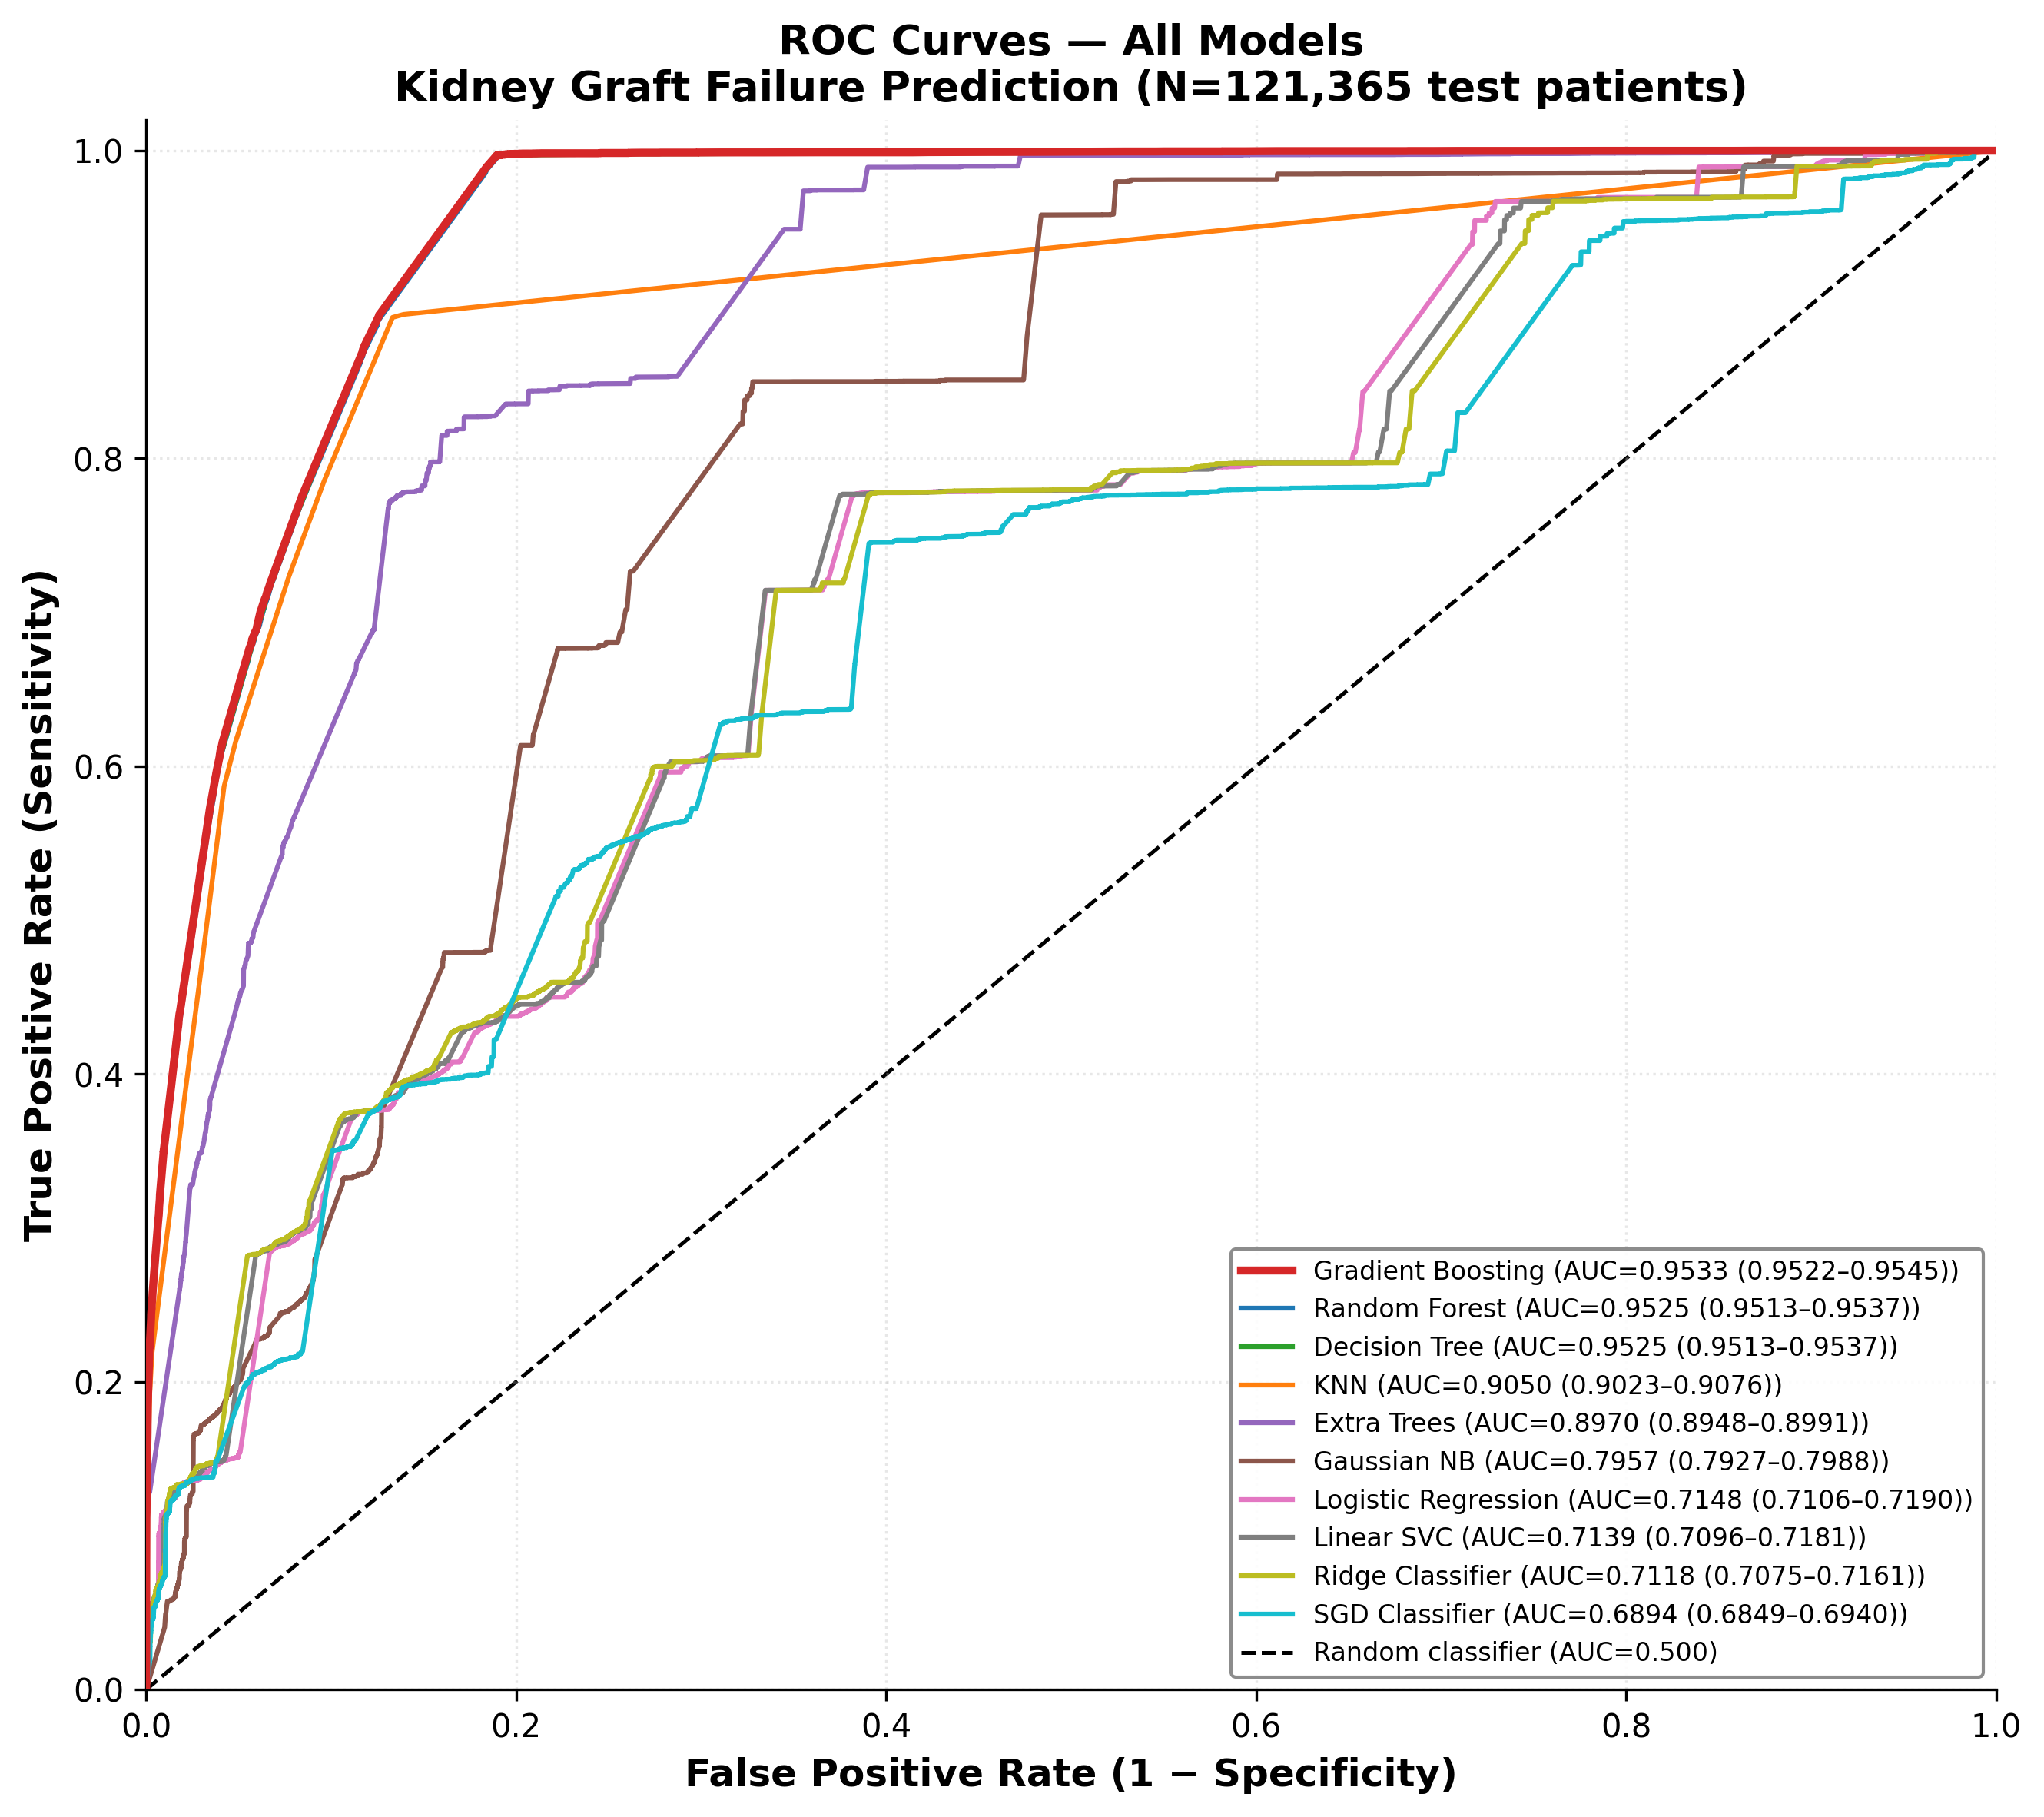
\includegraphics[width=\textwidth]{fig1_roc_curves_all_models.png}
        \caption{ROC curves for all evaluated models.}
        \label{fig:all_rocs}
    \end{subfigure}
    \hfill
    \begin{subfigure}[b]{0.48\textwidth}
        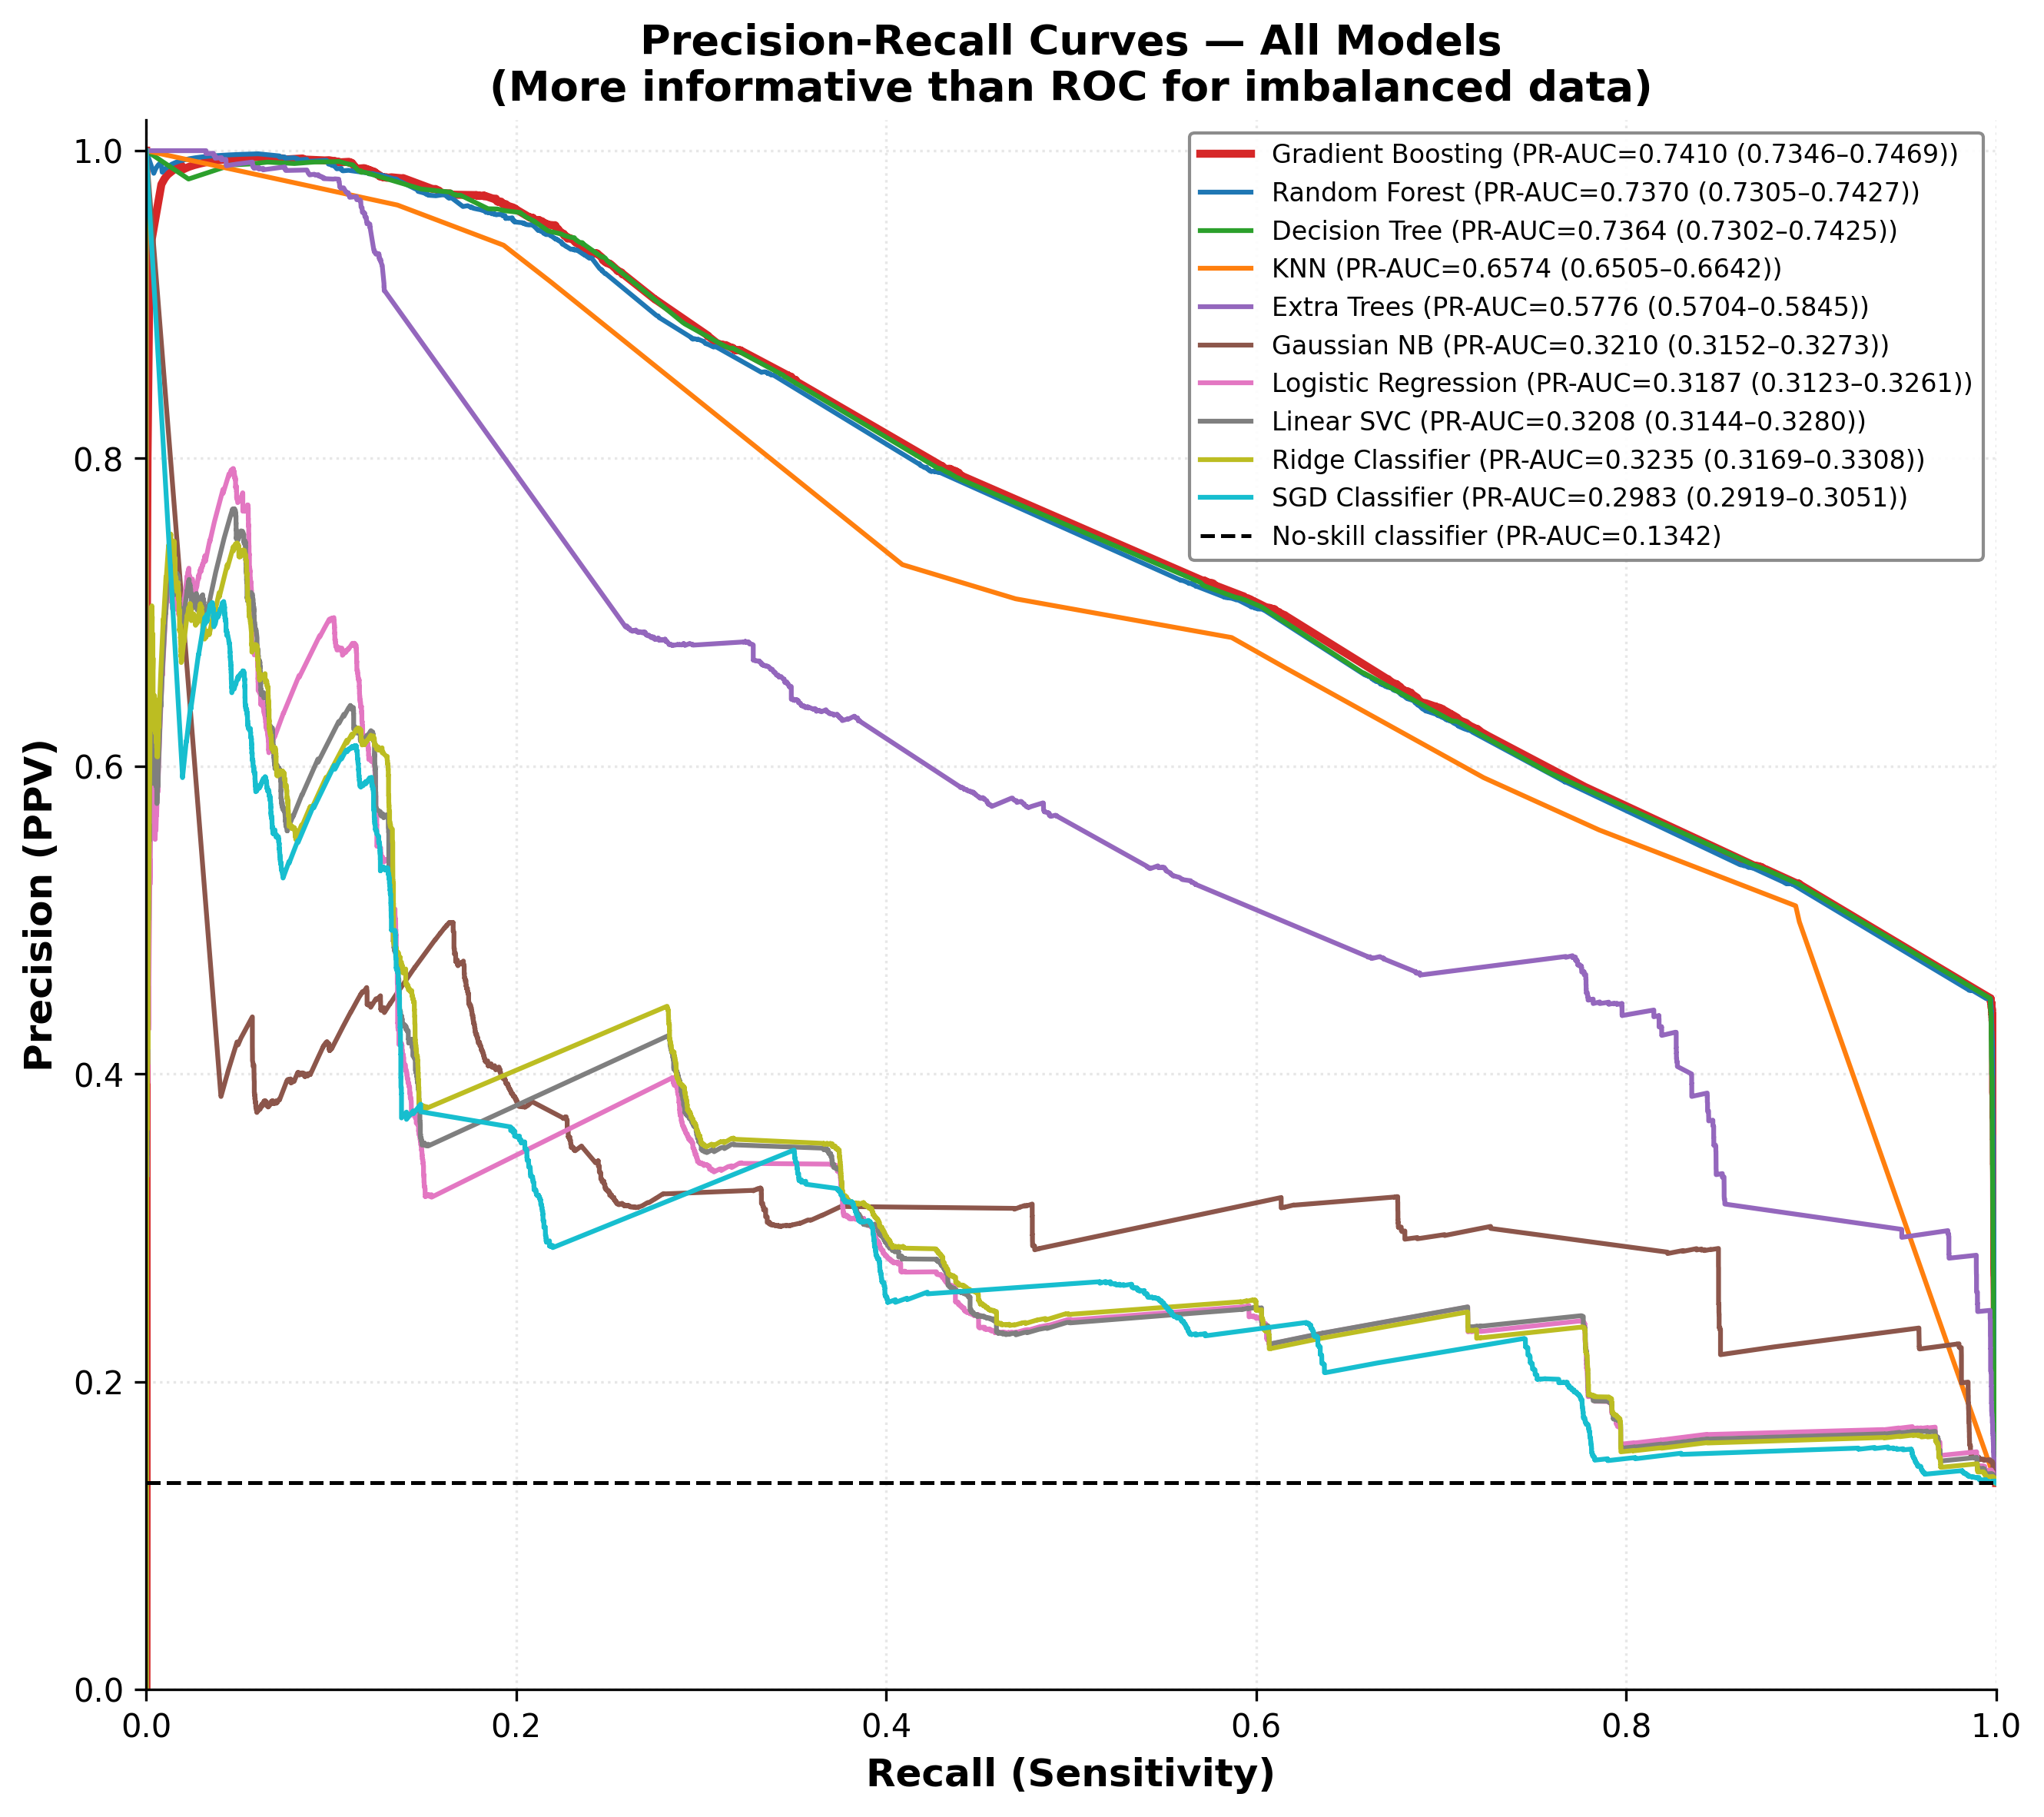
\includegraphics[width=\textwidth]{fig3_precision_recall_curves.png}
        \caption{Precision-recall curves for all evaluated models.}
        \label{fig:all_pr}
    \end{subfigure}
    \caption{Overall algorithm comparison across model families.}
    \label{fig:algorithm_comparison}
\end{figure}

At the selected threshold, the model achieved estimated positive predictive value (PPV) of approximately 24.3\% and negative predictive value (NPV) of 99.99\%, reflecting the low event prevalence and the model's excellent rule-out performance.

\subsection{Calibration and Clinical Utility}
Calibration curves confirmed that predicted probabilities aligned closely with observed graft failure rates across deciles, particularly in the upper risk range. The Brier score decomposition indicated strong calibration and good refinement. The decision curve analysis showed that the model provided net benefit above both treat-all and treat-none strategies across clinically meaningful thresholds.

\begin{figure}[H]
    \centering
    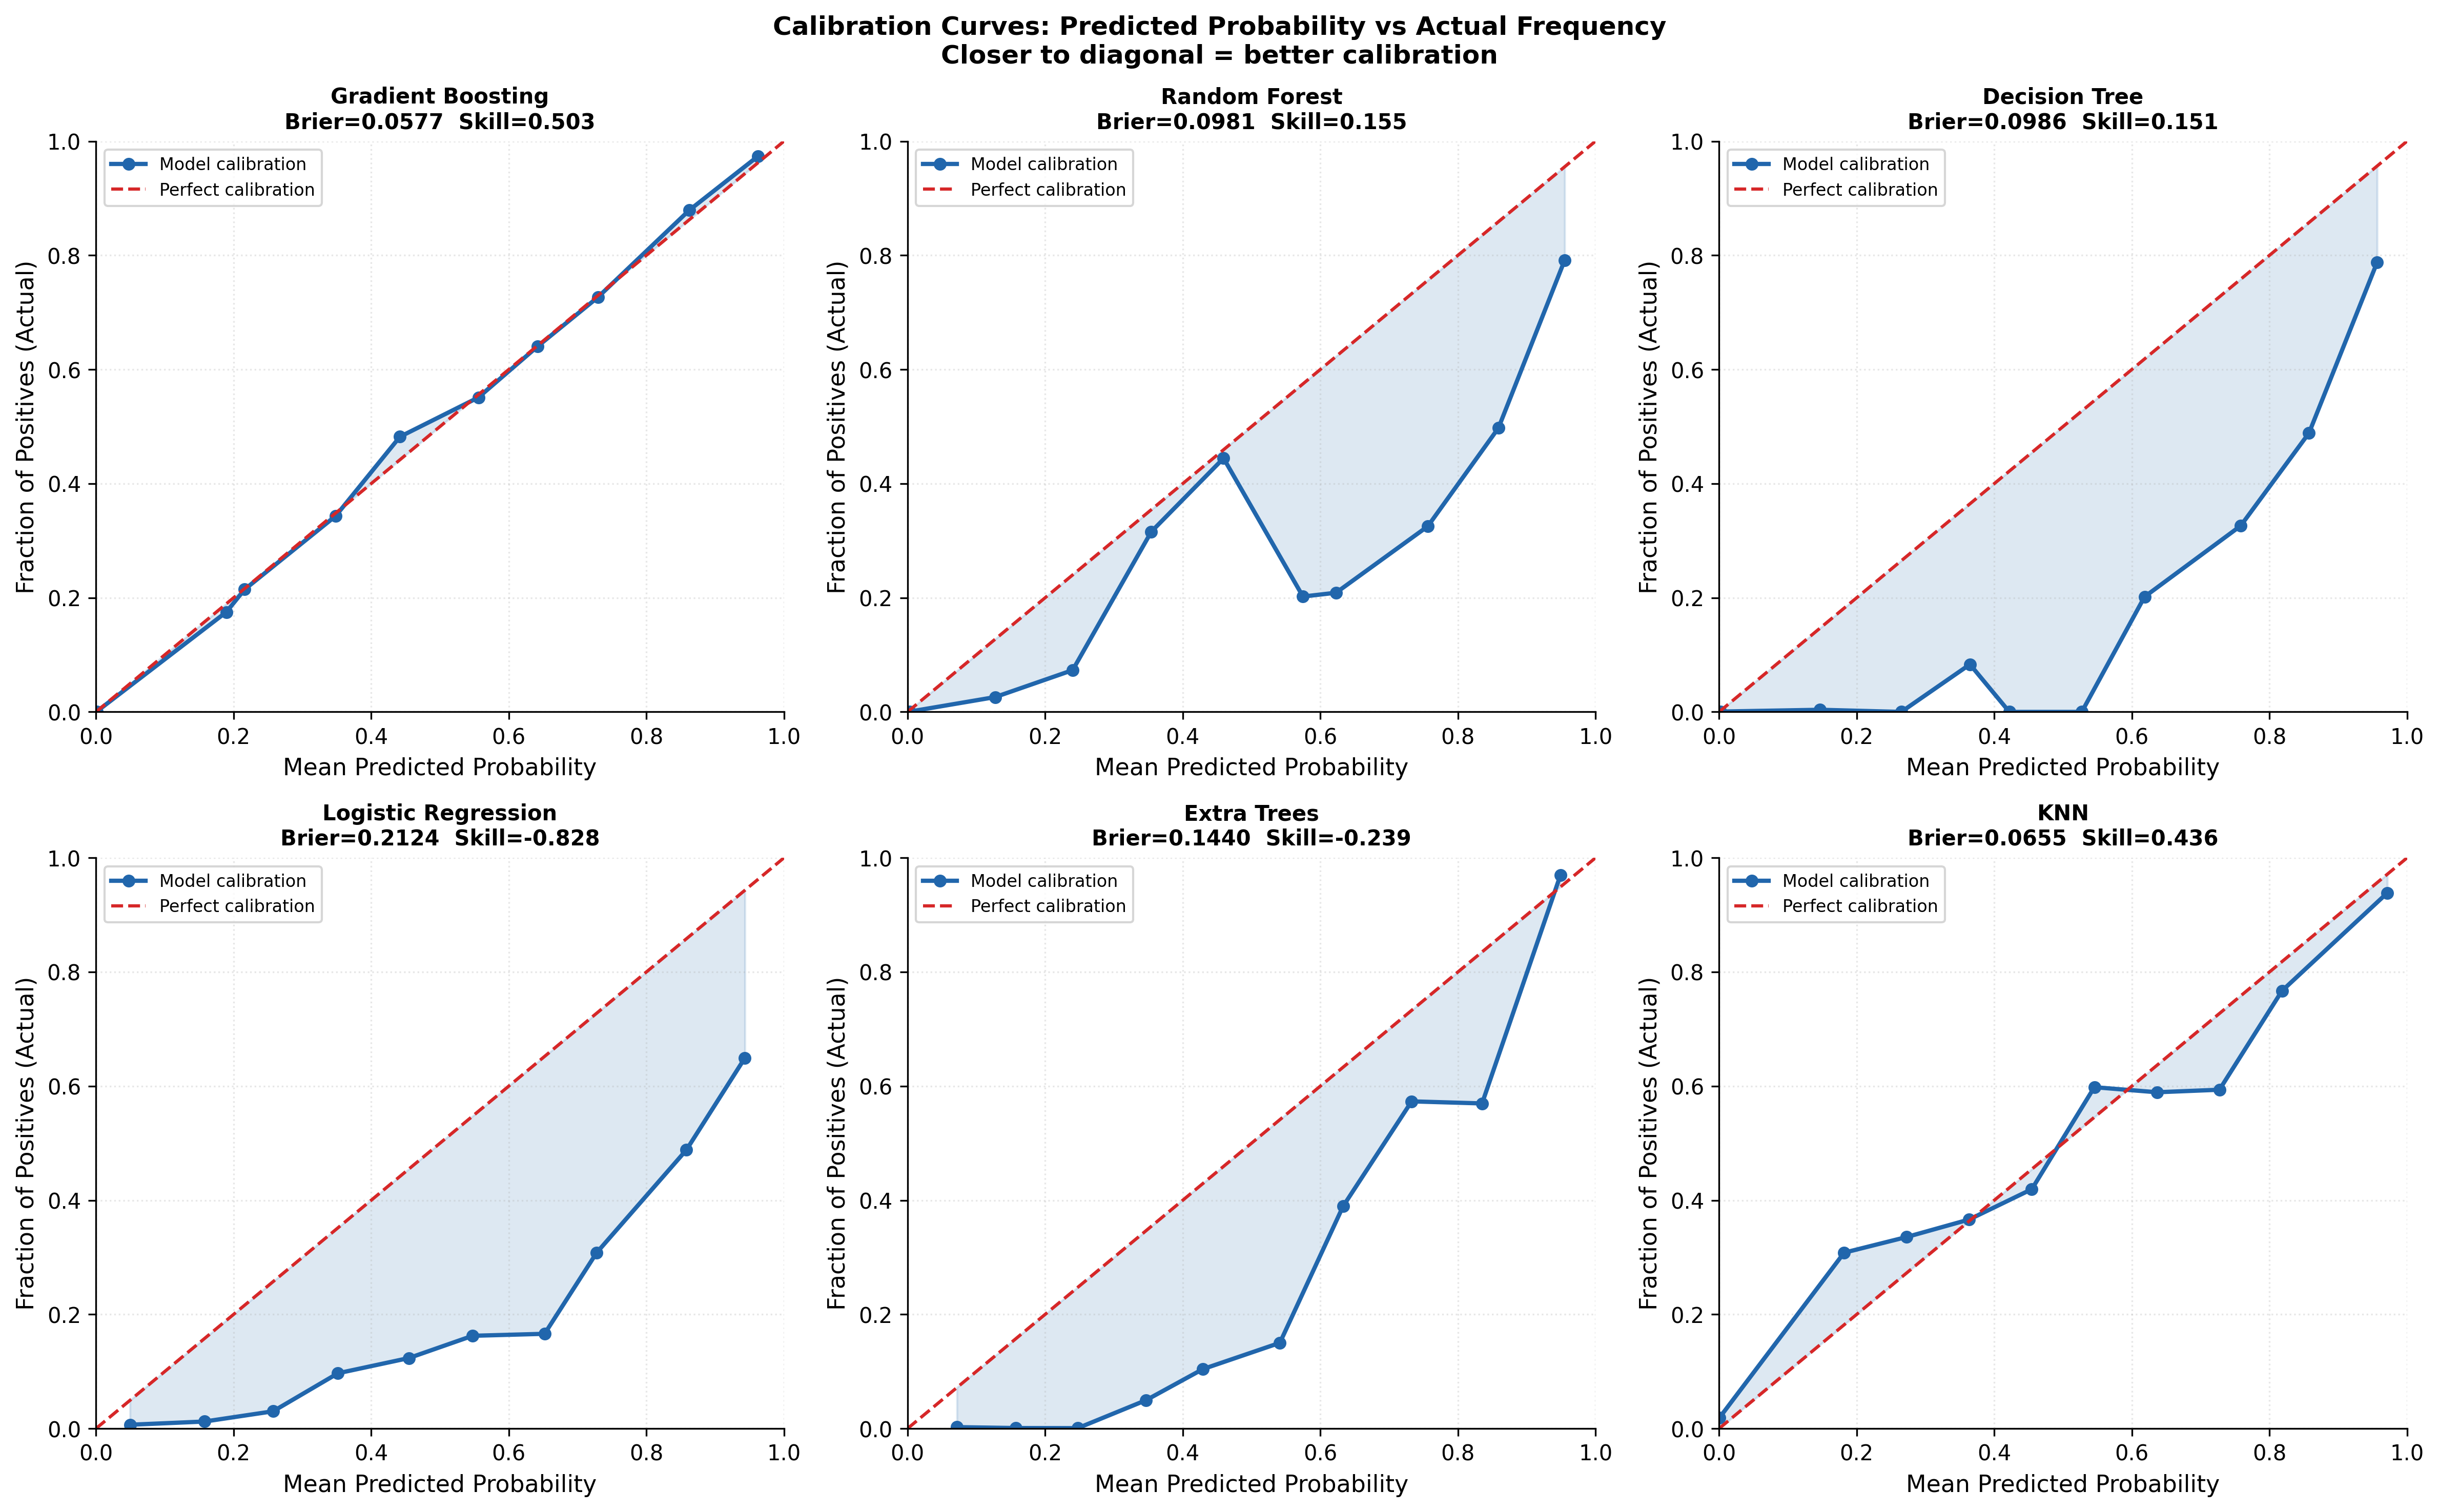
\includegraphics[width=0.75\textwidth]{fig1_calibration_curves.png}
    \caption{Calibration plot comparing predicted probabilities to observed graft failure incidence.}
    \label{fig:calibration}
\end{figure}

\subsection{Feature Importance via SHAP}
SHAP analysis identified serum creatinine as the dominant predictor. The summary beeswarm and importance plots demonstrated that serum creatinine contributed far more to risk than any other variable, with mean absolute SHAP values roughly 15 times greater than the second most important feature.

\begin{figure}[H]
    \centering
    \begin{subfigure}[b]{0.48\textwidth}
        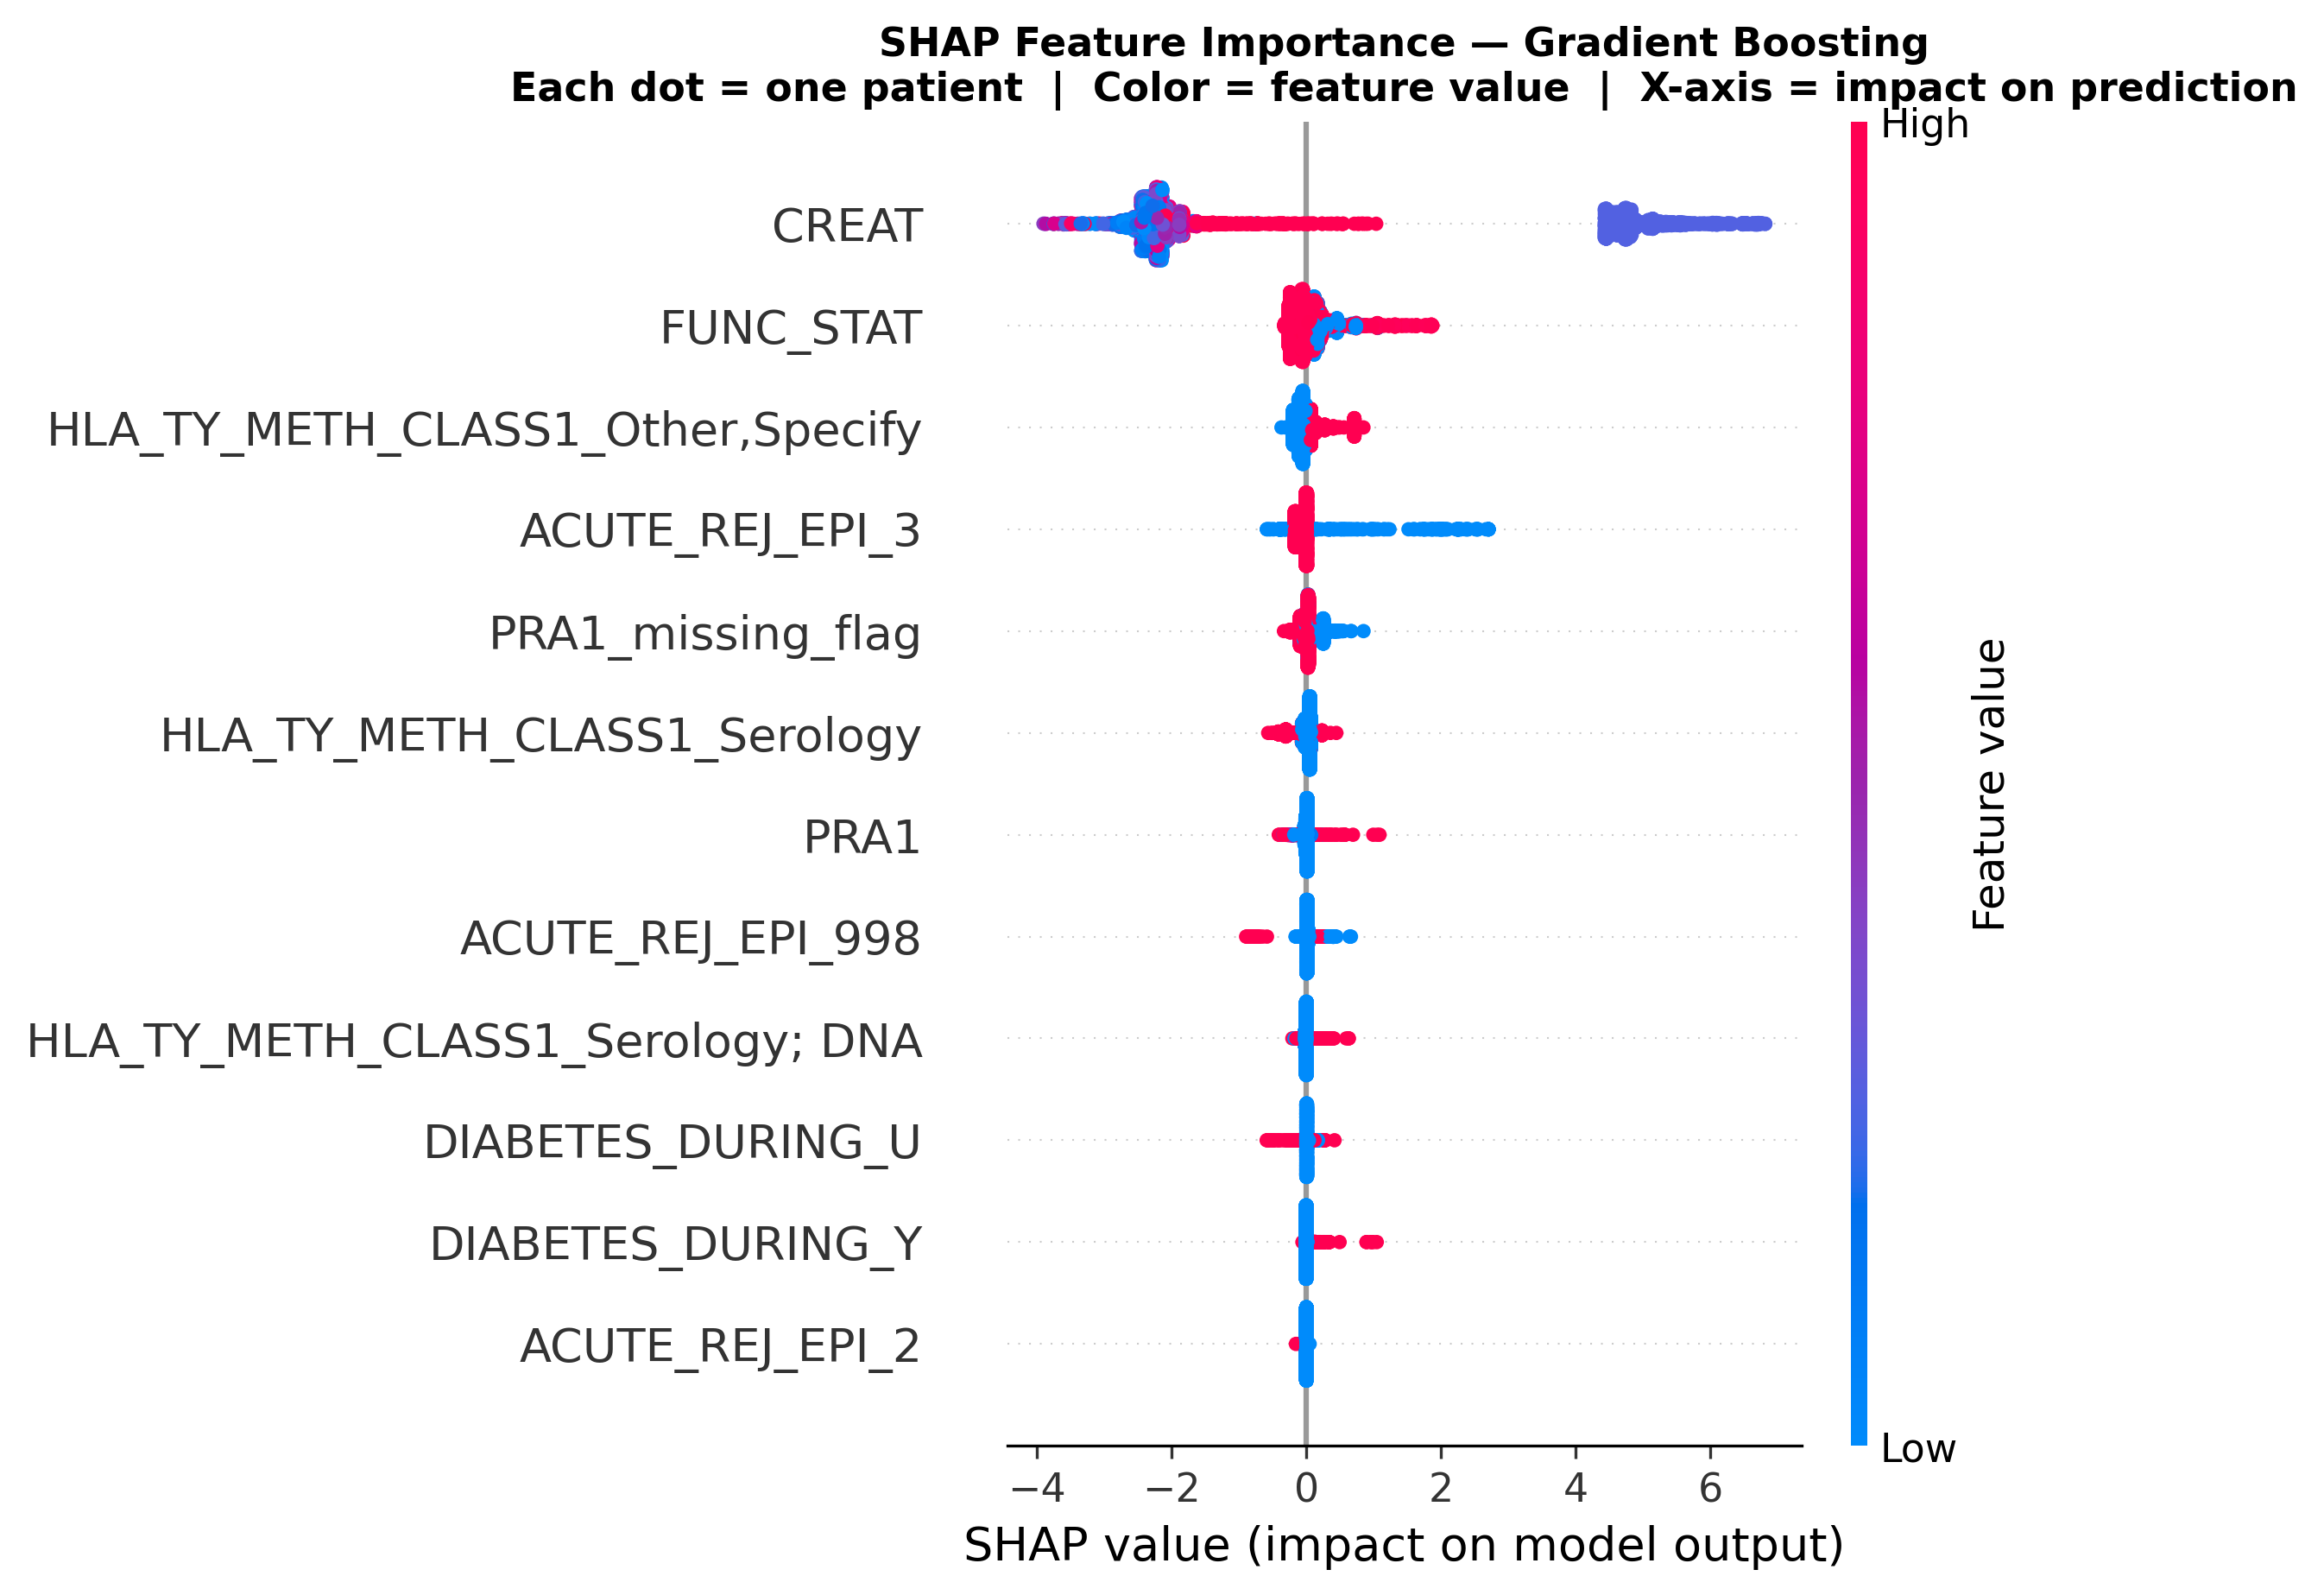
\includegraphics[width=\textwidth]{fig1_shap_beeswarm.png}
        \caption{SHAP beeswarm summary plot.}
        \label{fig:shap_beeswarm}
    \end{subfigure}
    \hfill
    \begin{subfigure}[b]{0.48\textwidth}
        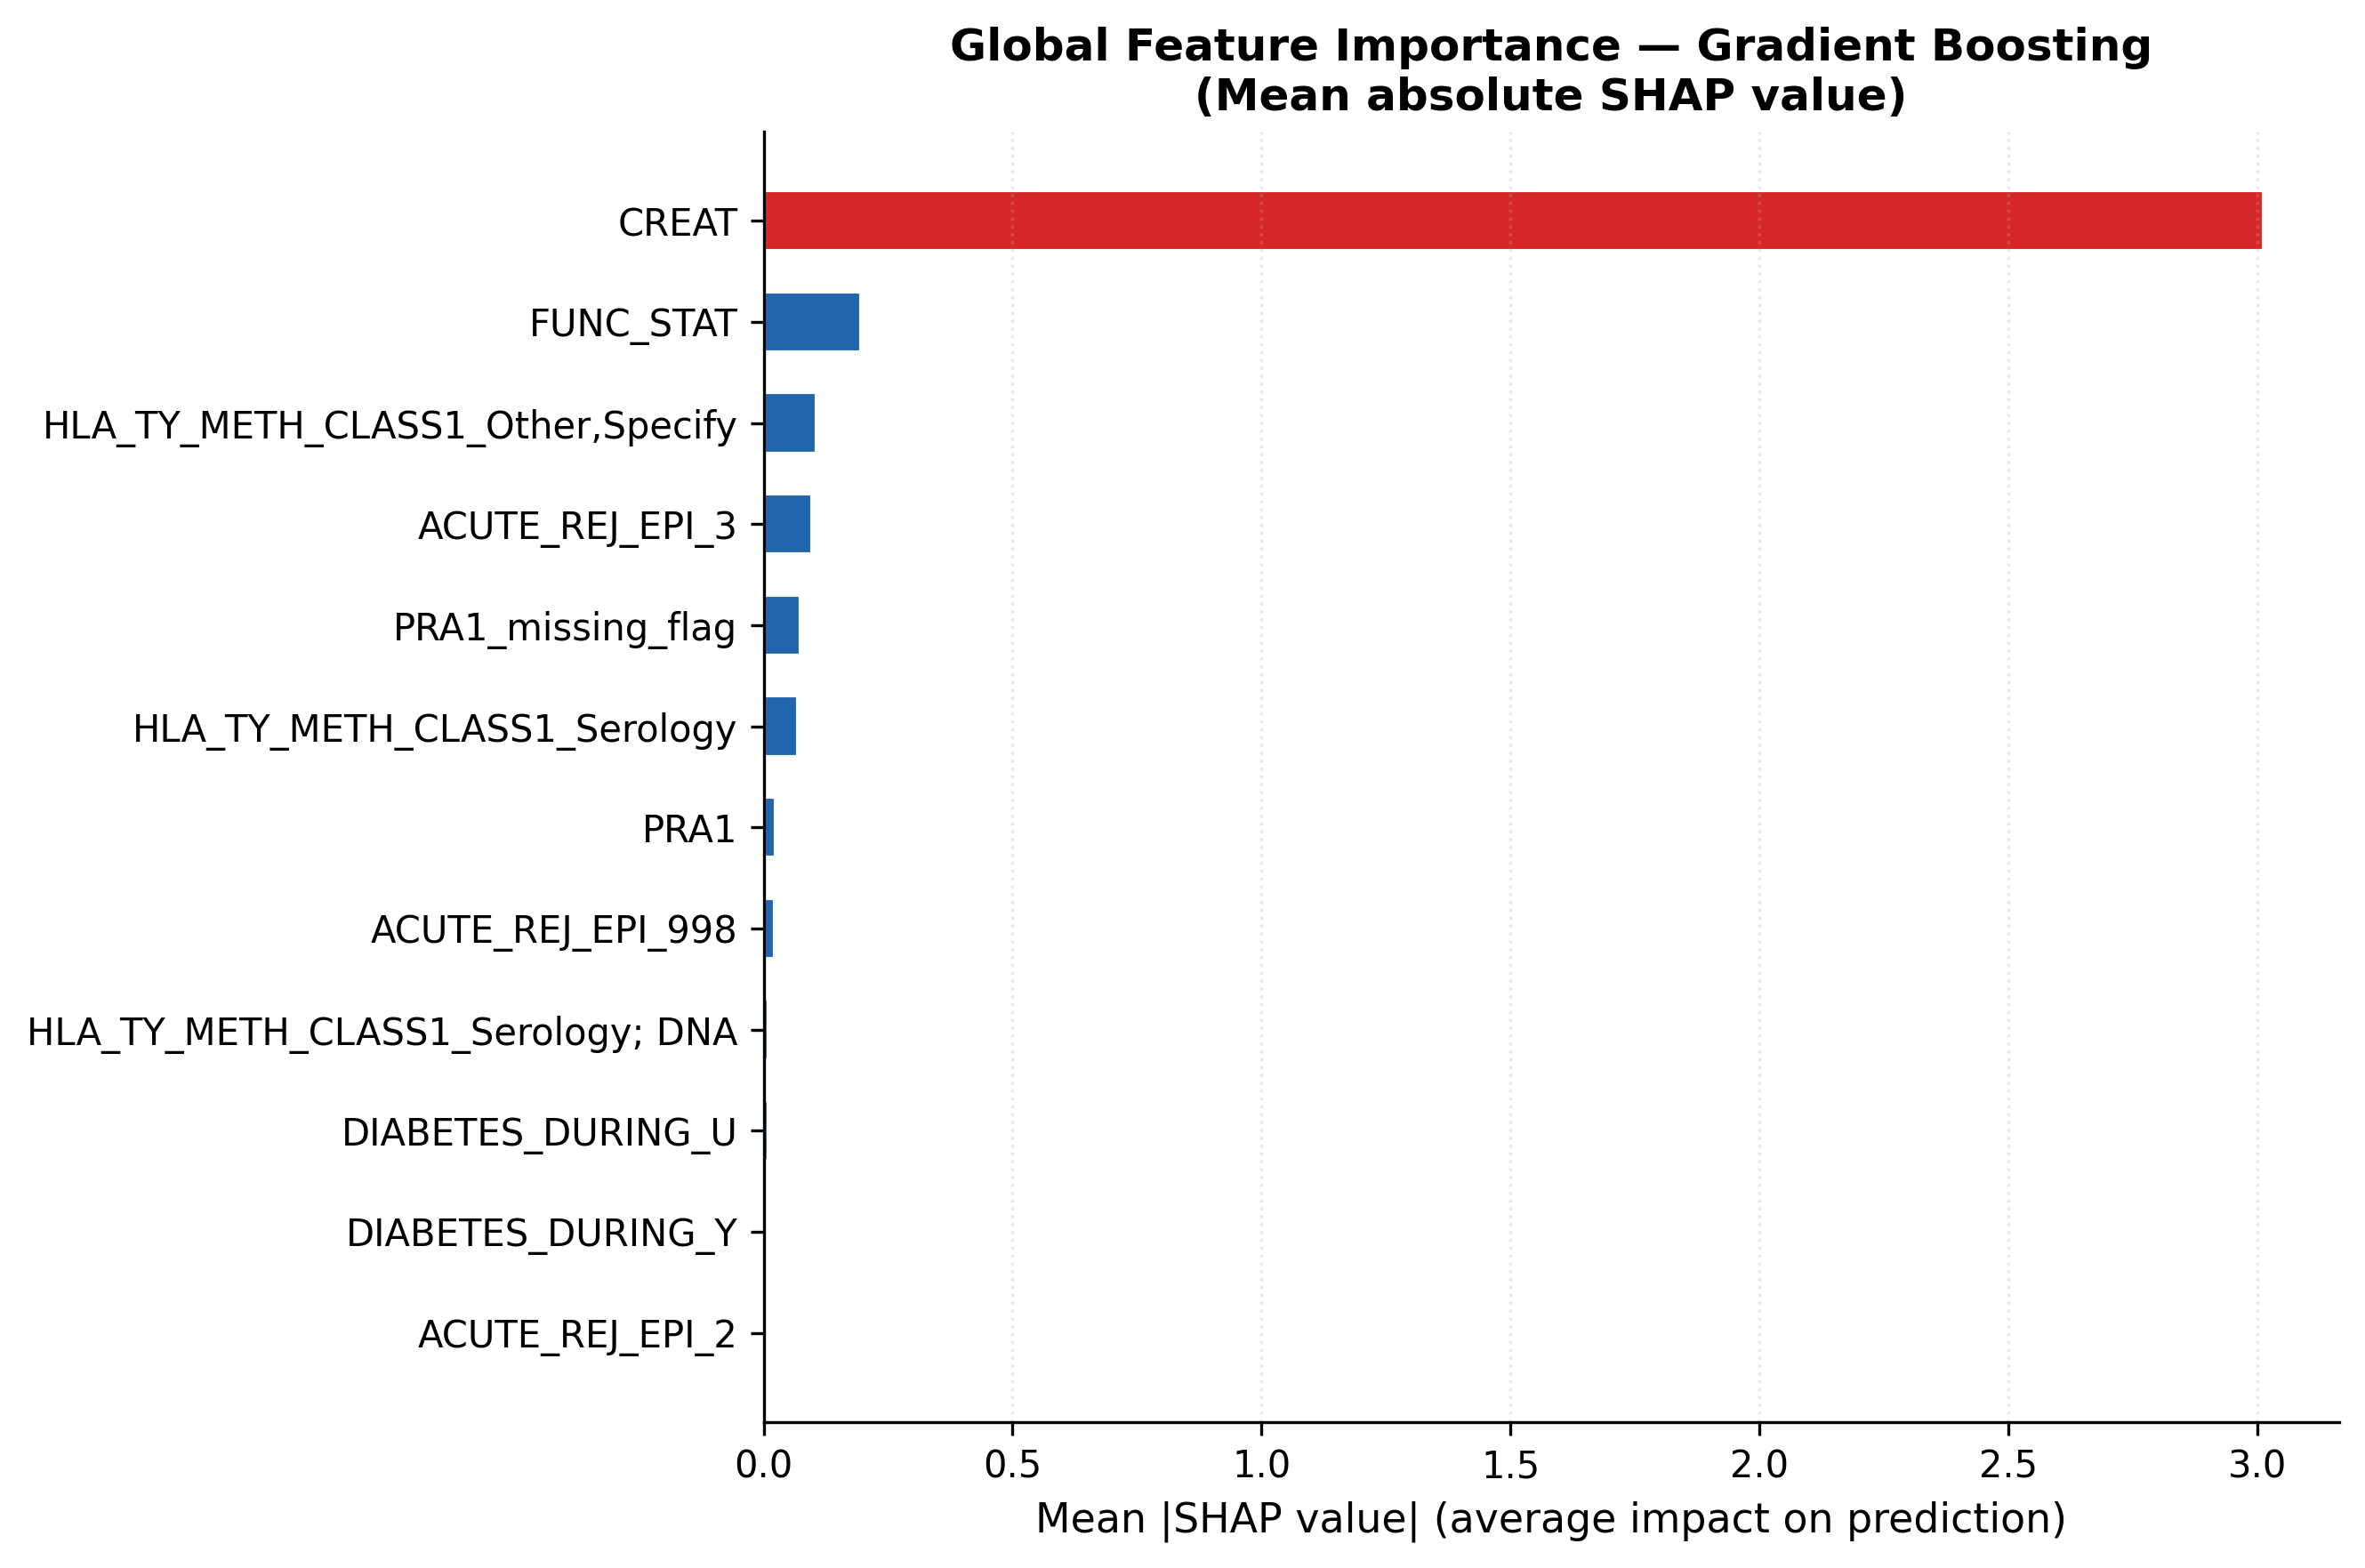
\includegraphics[width=\textwidth]{fig2_shap_importance.png}
        \caption{Feature importance ranking by mean |SHAP|.}
        \label{fig:shap_importance}
    \end{subfigure}
    \caption{Model explainability using SHAP.}
    \label{fig:shap}
\end{figure}

\subsection{Feature Interactions and Non-Linearity}
SHAP dependence and interaction analysis revealed non-linear risk patterns. In particular, risk increased sharply for recipients with creatinine levels above 2.5 mg/dL, and acute rejection episodes amplified this effect. The interaction plot in Figure \ref{fig:shap_interactions} highlights how the combined presence of elevated creatinine and rejection episodes produced outsized risk contributions.

\begin{figure}[H]
    \centering
    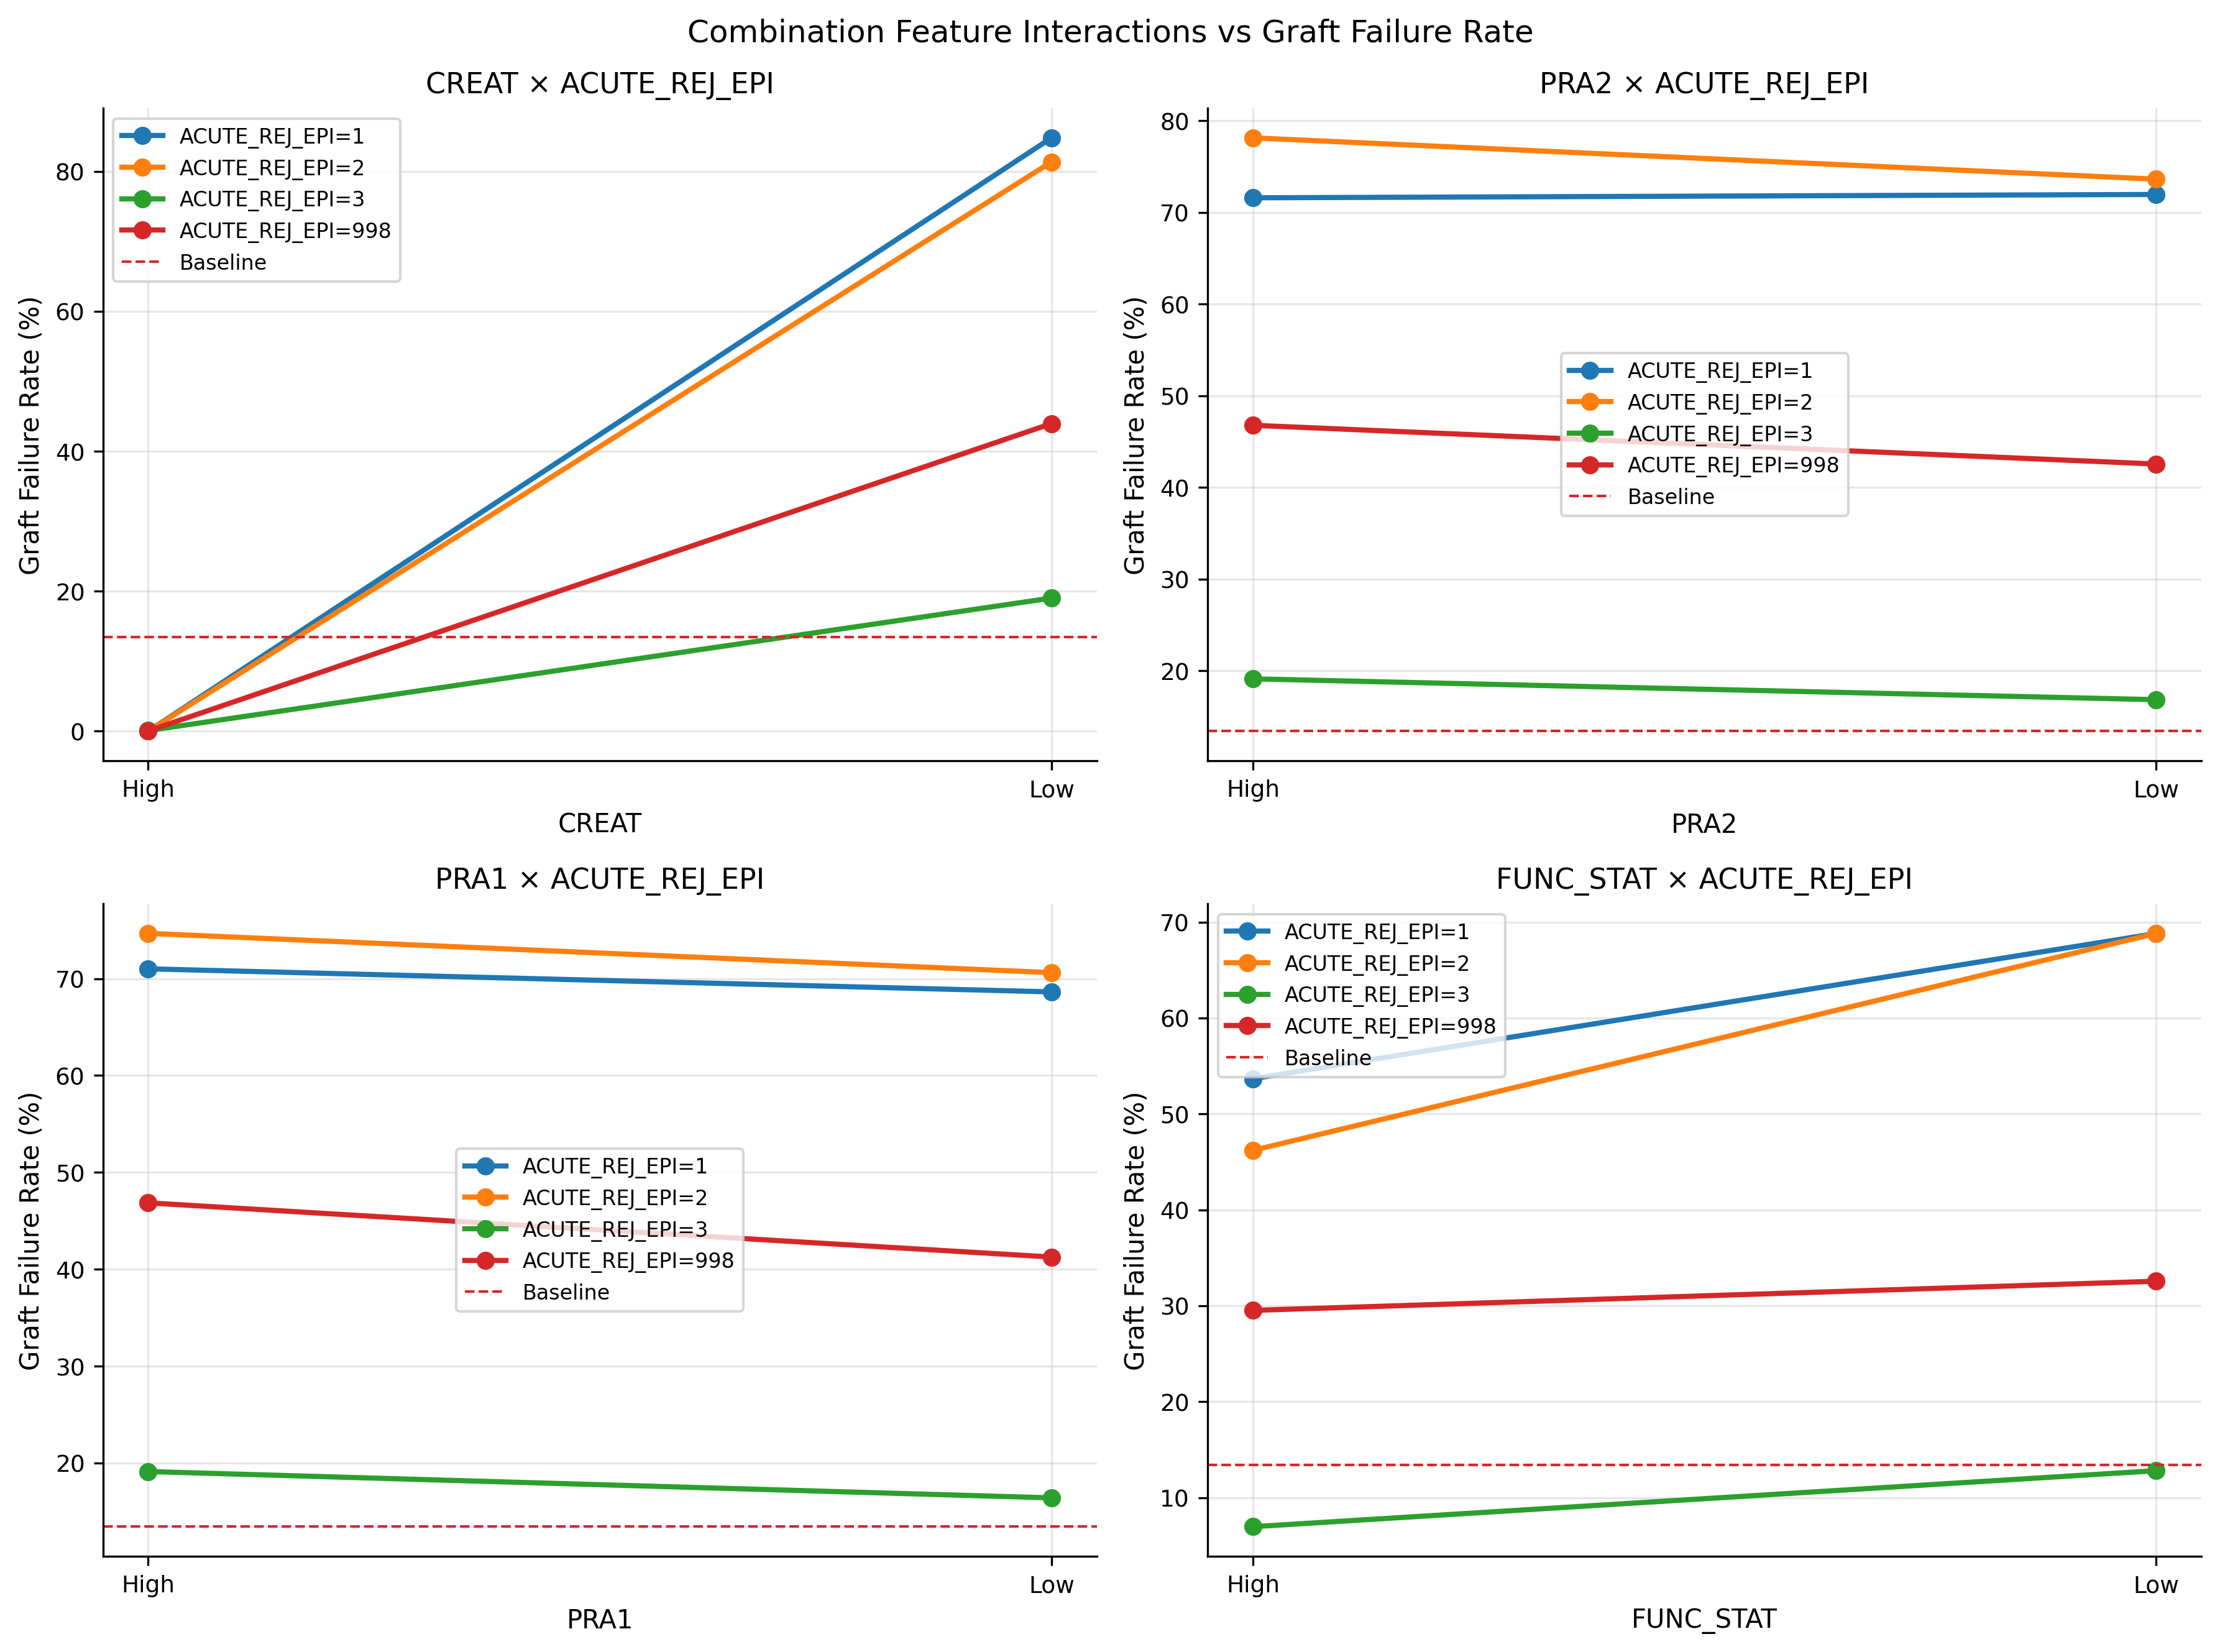
\includegraphics[width=0.75\textwidth]{fig3_combination_interactions.png}
    \caption{SHAP interaction analysis demonstrating non-linear synergy between serum creatinine and acute rejection.}
    \label{fig:shap_interactions}
\end{figure}

\subsection{Risk Stratification}
Predicted risk quartiles showed strong clinical separation. The low-risk quartile had an observed failure rate of 0.8\%, while the high-risk quartile had a failure rate of 23.4\%. This 29-fold gradient supports using model scores to tailor follow-up intensity.

\begin{table}[H]
\centering
\caption{Observed Graft Failure Rates by Predicted Risk Quartile}
\label{tab:quartiles}
\small
\begin{tabular}{lccc}
\toprule
\textbf{Risk Quartile} & \textbf{N} & \textbf{Failure Rate} & \textbf{95\% CI} \\
\midrule
Low Risk & 30,341 & 0.8\% & 0.68--0.92\% \\
Intermediate-Low Risk & 30,341 & 3.2\% & 2.84--3.56\% \\
Intermediate-High Risk & 30,341 & 10.5\% & 10.02--11.00\% \\
High Risk & 30,342 & 23.4\% & 22.68--24.12\% \\
\bottomrule
\end{tabular}
\end{table}

\begin{figure}[H]
    \centering
    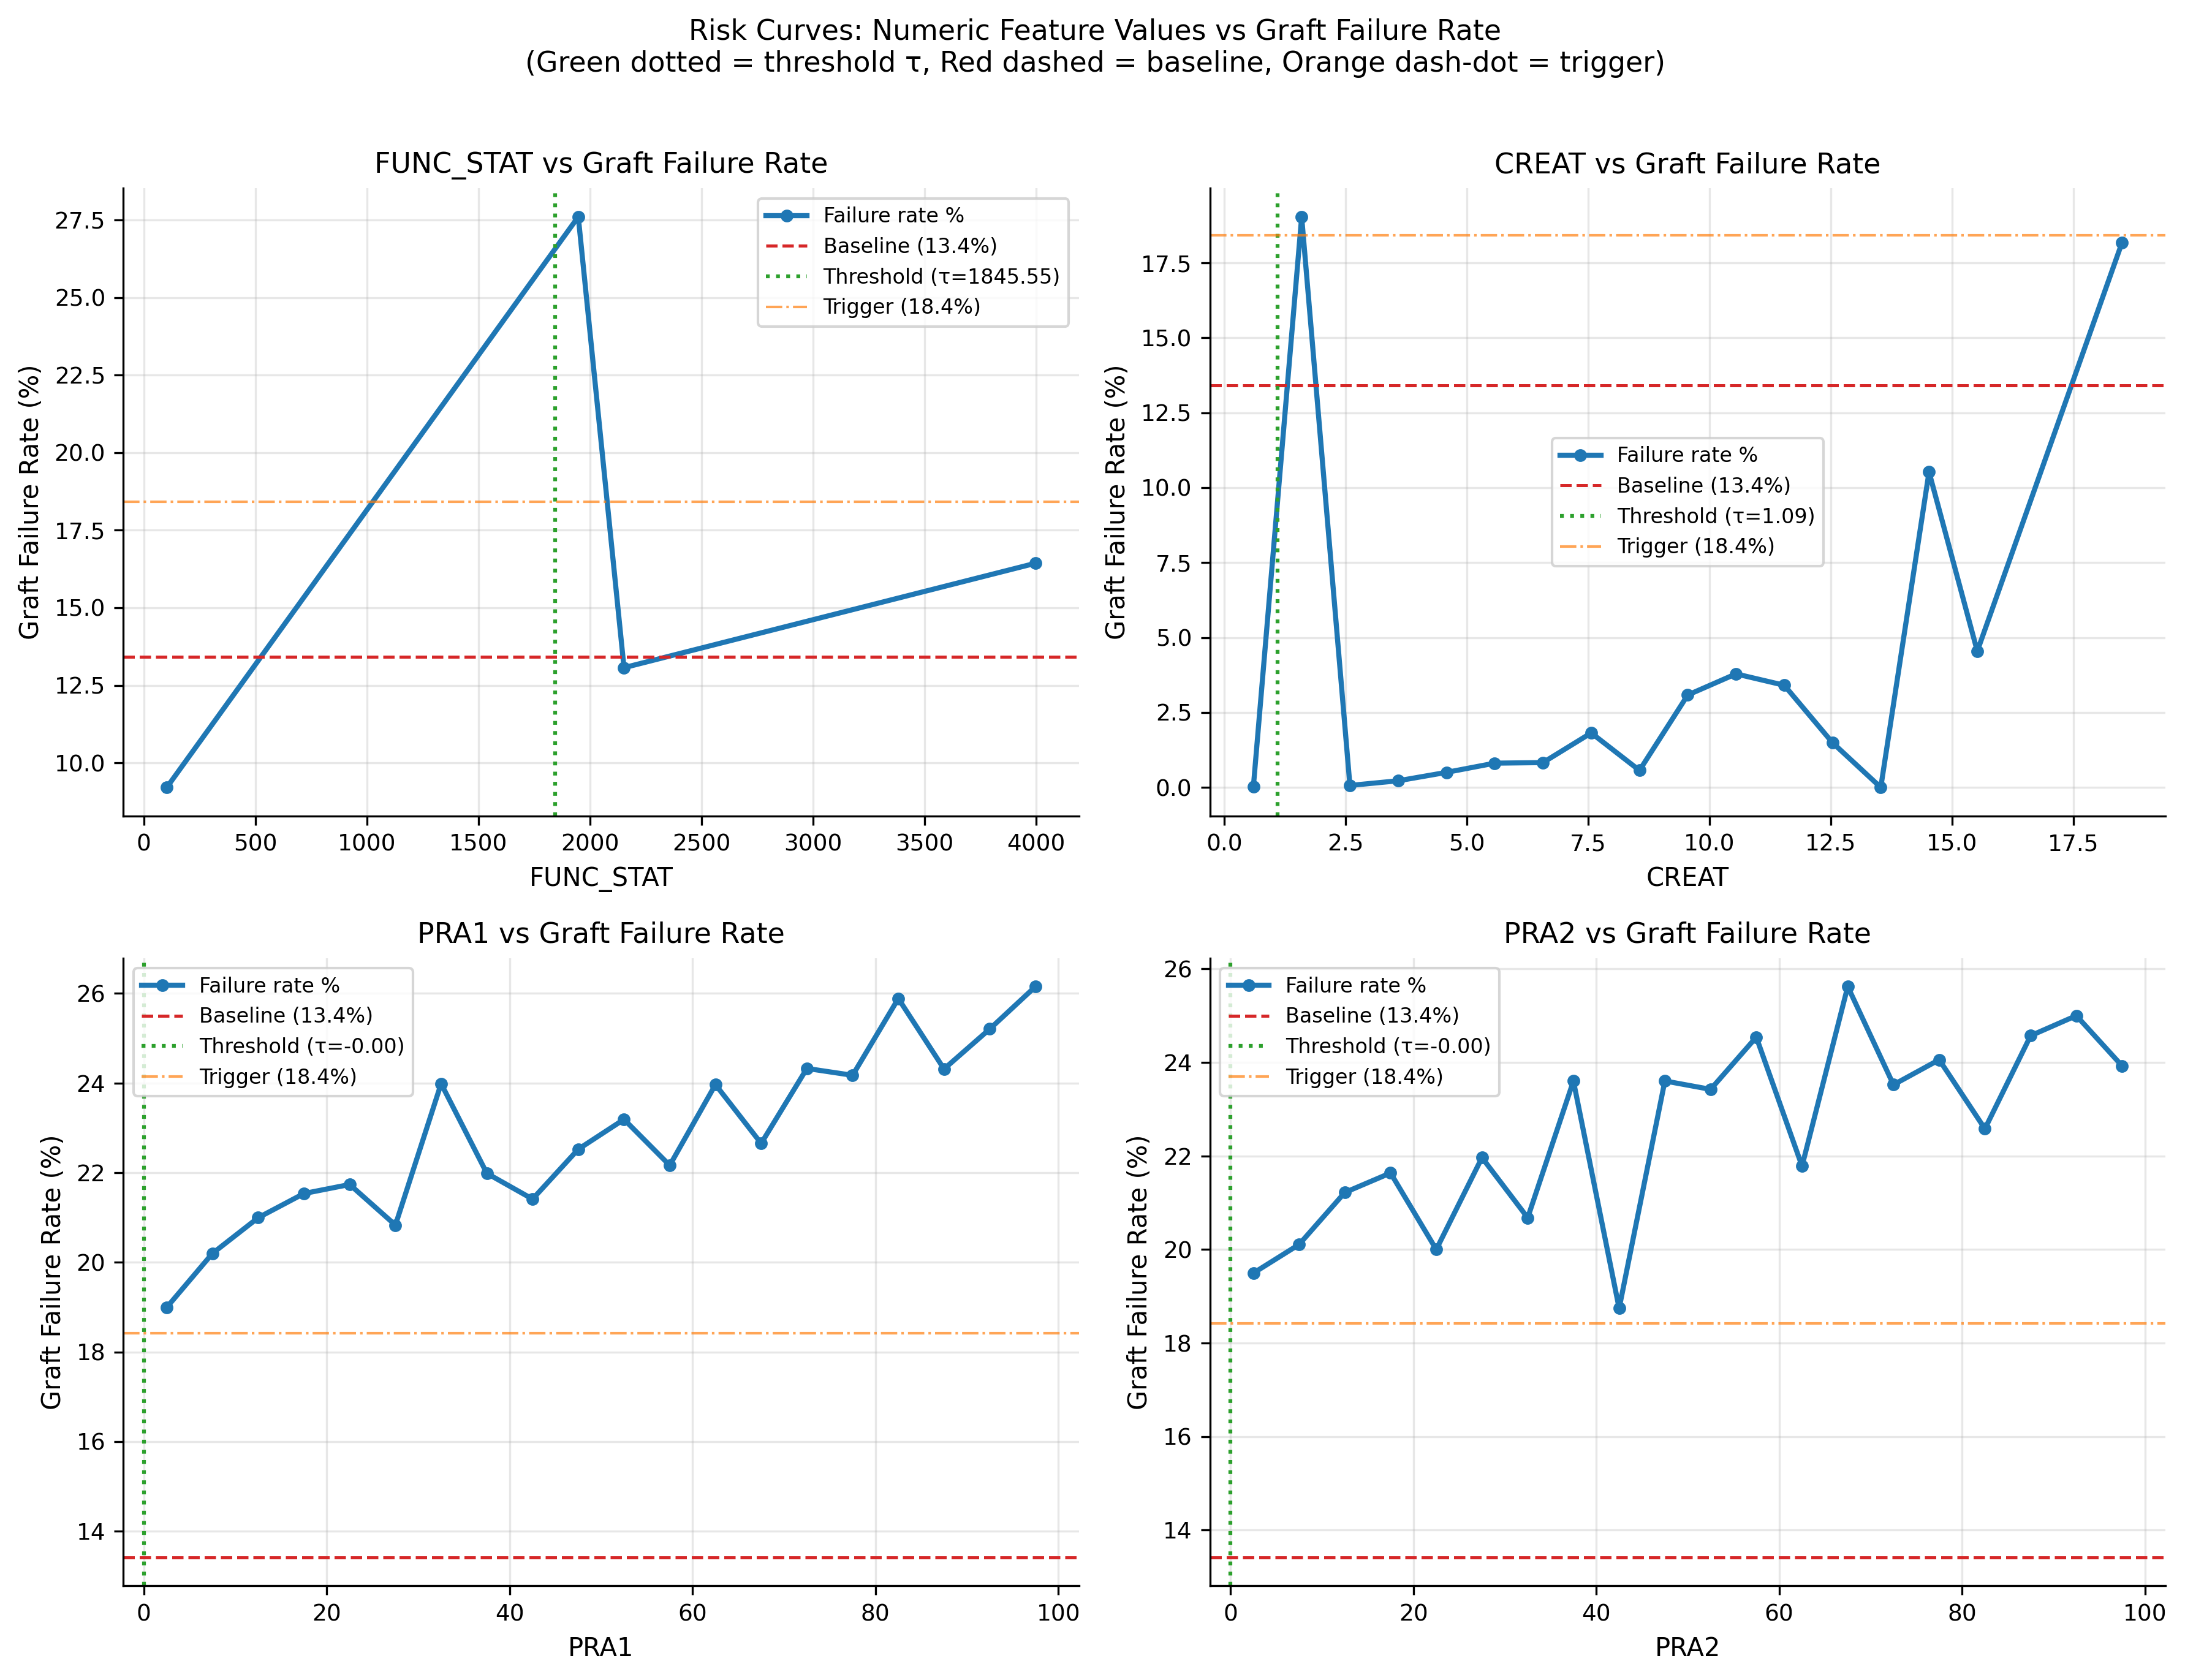
\includegraphics[width=0.75\textwidth]{fig1_numeric_risk_curves.png}
    \caption{Risk stratification curves showing increasing observed failure incidence across predicted risk quantiles.}
    \label{fig:risk_stratification}
\end{figure}

\begin{table}[H]
\centering
\caption{Key Model Performance Metrics on the Held-Out Test Set (N=121,365)}
\label{tab:metrics}
\small
\begin{tabular}{lc}
\toprule
Metric & Value \\
\midrule
ROC-AUC & 0.9533 (95\% CI 0.9522--0.9545) \\
Precision-Recall AUC & 0.850 \\
Sensitivity & 99.69\% (99.61--99.78\%) \\
Specificity & 81.05\% (80.82--81.29\%) \\
Brier Score & 0.0577 \\
\bottomrule
\end{tabular}
\end{table}

\subsection{Secondary Insights}
The SHAP analysis also revealed non-linear effects for functional status and acute rejection. For example, recipients with lower functional status had disproportionately higher predicted risk, while PRA1 missingness carried independent prognostic value beyond the recorded antibody level.

\section*{Acknowledgments}
The authors acknowledge the UNOS STAR data repository and the data science team supporting model development.

\bibliographystyle{plainnat}
\begin{thebibliography}{9}
\bibitem{Wolfe1999} Wolfe, R. A., et al. (1999). Comparison of mortality in all patients on dialysis, patients on dialysis awaiting transplantation, and recipients of a first cadaveric transplant. \textit{New England Journal of Medicine}, 341(23), 1725--1730.
\bibitem{Hart2019} Hart, A., et al. (2019). OPTN/SRTR 2018 Annual Data Report: Kidney. \textit{American Journal of Transplantation}, 20(S1), 20--129.
\bibitem{Halloran2004} Halloran, P. F., et al. (2004). Identifying subgroups of kidney transplant recipients at high risk for late donor-specific antibody formation associated with allograft loss. \textit{Clinical Journal of the American Society of Nephrology}, 8(12), 2262--2272.
\bibitem{Rajkomar2018} Rajkomar, A., et al. (2018). Scalable and accurate deep learning with electronic health records. \textit{Nature Medicine}, 24(3), 338--342.
\bibitem{DeLong1988} DeLong, E. R., et al. (1988). Comparing the areas under two or more correlated receiver operating characteristic curves. \textit{Biometrics}, 44(3), 837--845.
\bibitem{Lundberg2017} Lundberg, S. M., \& Lee, S. I. (2017). A unified approach to interpreting model predictions. In \textit{Advances in Neural Information Processing Systems} (pp. 4765--4774).
\end{thebibliography}

\end{document}
